\chapter{Специи}
\section{Универсальный язык хорошего вкуса}

Итак, сегодня раскрываю секреты\ldots которые секретами не являются.
Как же сделать пресное блюдо привлекательным? 
Очень просто: наделить его всеми шестью вкусами — солёным, сладким, кислым, горьким, вяжущим и острым. На этом всё, спасибо за внимание, до свидания\ldots Шучу, читаем дальше!

Как известно, в ведической традиции считается, что основная трапеза должна содержать все 6 вкусов. Я с этим утверждением абсолютно солидарен, хоть и не приветствую соль. Когда эти вкусы гармонично взаимодействуют, человек получает весь спектр эмоций, потому что по сути, вкус~--- это эквивалент эмоции, и как только вы поймёте это, вам станет ясно, почему иногда хочется шоколадки, а иногда и хрена с чесноком. В другом случае, это потребность физиологического характера, например в период очищения или дефицита определённых веществ.

Так вот. Есть блюда, любимые многими, такие как плов, например. Я здесь не рассматриваю мясо, потому что с ним можно хоть гвозди есть, всё равно будет вкусно. Речь о вегетарианском варианте. Чтобы вы поняли, что делает безвкусный рис таким вкусным, надо просто проанализировать состав плова:
\begin{itemize}
\item Соль — солёный
\item Морковь, изюм, курага и чернослив — сладкий
\item Барбарис — кислый
\item Куркума, шафран — горький
\item Кумин — вяжущий
\item Лук и чеснок — острый
\item ну и Рис между делом, как сорбент всей композиции
\end{itemize}

Я думаю, вы теперь поняли, что рис без специй будет напоминать что-то вроде риса из студенческой столовки. Плов не самый лучший пример, но показательный. Я не считаю рис достойным продуктом для употребления, но на востоке в этом очень преуспели.

Теперь вы можете понять почему базу составляют всего несколько специй.

Другой пример — салат с рукколой и черри. Здесь всё дело в соусе по тому же принципу:
\begin{itemize}
\item оливковое масло, 2 стл
\item лимонный сок, 2 стл — кислый
\item гранатовый соус или шиповника, 1 стл — сладкий
\item чёрный перец, щепотка — острый
\item прованские травы, 1 чл — вяжущий
 
\item руккола — горький
\item сушёные помидоры — солёный
\end{itemize}


Заправка для Греческого салата:
\begin{itemize}
\item 3 чл оливкового масла
\item 3 чл лимонного сока
\item 1 зуб чеснока
\item 1/4 чл орегано
\item 1/4 чл соли
\item Сладость даёт болгарский перец
\end{itemize}

Ещё один вариант соуса:
\begin{itemize}
\item Растительное масло, 2 стл
\item Чеснок, 4 зуб.
\item Соевый соус, 4 стл
\item Лимонный сок, 2 чл
\item Мёд, 1 чл
\item Черный перец, 2 щеп.
\item Зелень, горсть.
\end{itemize}

Как вы видите, соусы содержат в себе почти все вкусы, а недостающие восполняют овощи и фрукты. Вообщем, принцип понятен.

Я заметил, что добавляя в блюдо чеснок, оно буквально преображается. Можно долго рассуждать о его раджастической природе, что это продукт в гуне невежества и прочее-прочее, но мы живём на земле, в конце концов. Особо просветлённые могут заменить его асафетидой. Чеснок, горький и острый одновременно, делает блюдо аппетитнее, это факт. В ресторанах вместе с лавашом часто подают пиалу с чесночным маслом. А на столе всегда есть соль, сахар и перец и лимон.

Специи~--- самый доступный способ сделать блюдо богаче. Только не сублимируйте эмоциональный вакуум — любимое дело гораздо важнее еды! Любите себя и дарите любовь.


\begin{figure}[ht]
    \centering
    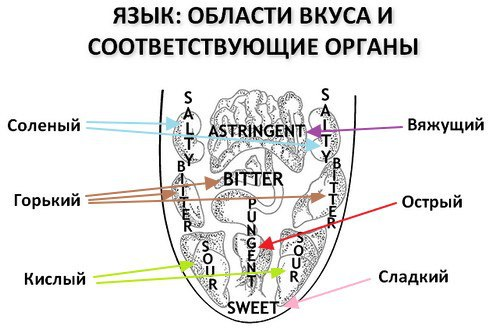
\includegraphics[width=0.6\textwidth]{img/SixTastes}
    \label{fig:1}
\end{figure} 

\section{Про специи}
Сейчас я я хотел бы поговорить о специях и о том, как их выбирать и хранить. Об их свойствах я рассказывать не буду, потому что это долго, неинтересно и больше про лечебные свойства, что в наш динамичный мир не вписывается. Поскольку большинство людей — заложники вкуса, то лишь его и обозначу. Ниже перечислю основные специи, как говорится must-have, которые должны быть всегда под рукой.

\subsection{База}
\begin{itemize}
\item Кумин (зира) — вяжет: в основном, для бобовых.
\item Кориандр (семена кинзы) — для овощей и нотки «бородинского».
\item Корица — делает всё слаще.
\item Чили — жгучая острота.
\item Чёрный перец — грубая острота.
\item Ванильный сахар — делает выпечку сексуальнее.
\item Соль — делает так, что хочется ещё.
\item Сахар — без комментариев.
\item Мёд — сладость без вреда.
\item Лимон — добавляет кислинку.
\item Чеснок — делает всё аппетитнее, остро-горький.
\item Зелень (кинза, петрушка, укроп, руккола) — вкус, аромат и полезная горечь.
\end{itemize}

\subsection{На редкий случай}
\begin{itemize}
\item Куркума — для овощей.
\item Гвоздика — для выпечки.
\item Мускат — универсален.
\item Имбирь — острый, универсален.
\item Бадьян — пряный, для напитков.
\item Хмели-сунели — для каш.
\item Розовый перец — для супа.
\item Прованские травы — для салатов.
\item Орегано — для помидоров.
\item Лавровый лист — для супа.
\end{itemize}

\subsection{Целые или молотые}
Целые предпочтительнее, т. к. дольше сохраняют аромат и вкус. Поэтому лучше иметь кофемолку и молоть самостоятельно. Однако есть специи, которые смолоть в обычной кофемолке не получится, поэтому надо брать готовый вариант. Обычно это Корица, Мускат, Куркума и другие твёрдые виды.

\subsection{Как выбирать и где покупать}
Лучшие специи, на мой скромный взгляд, производит компания TRS. Приобрести их вы можете здесь: http://indianspices.ru или любом другом магазине специй. Если нет TRS, берите любые в герметичной упаковке. Всё, что продаётся на рынках в открытом виде — давно выветрилось и интереса не представляет.

\subsection{Как хранить}
Самое простое — в аптечных контейнерах (видел также в Ашане по 15р/шт). Купите по одному большому для каждой отдельной специи. Это дёшево и практично. Всё остальное — маркетинг. В таком виде они хранятся указанный на упаковке срок.
Если блюдо содержит смесь специй, как плов или пряники, то композицию лучше готовить непосредственно перед закладкой.

\subsection{Где купить специи}
\begin{itemize}
\item Специи: http://indianspices.ru
\item Специи: http://ashaindia.ru/indiyskie-specii/
\item Гималайская соль: http://hpcsalt.ru
\end{itemize}

% -------
% Здесь я просто делюсь своим опытом. Большинство людей блуждают в потёмках невежества и до сих пор употребляют плоть животных. Надеюсь, что публикуемые рецепты вдохновят вас подняться на ступень выше, и взглянуть на свой рацион трезво.
% 
% Завтра я расскажу вам маленький секрет хорошего соуса, овладев которым, вы сможете сделать любое блюдо аппетитным… и объясню, почему в базу вошли указанные специи.

\section{Про названия специй}

\begin{figure}[ht]
    \centering
    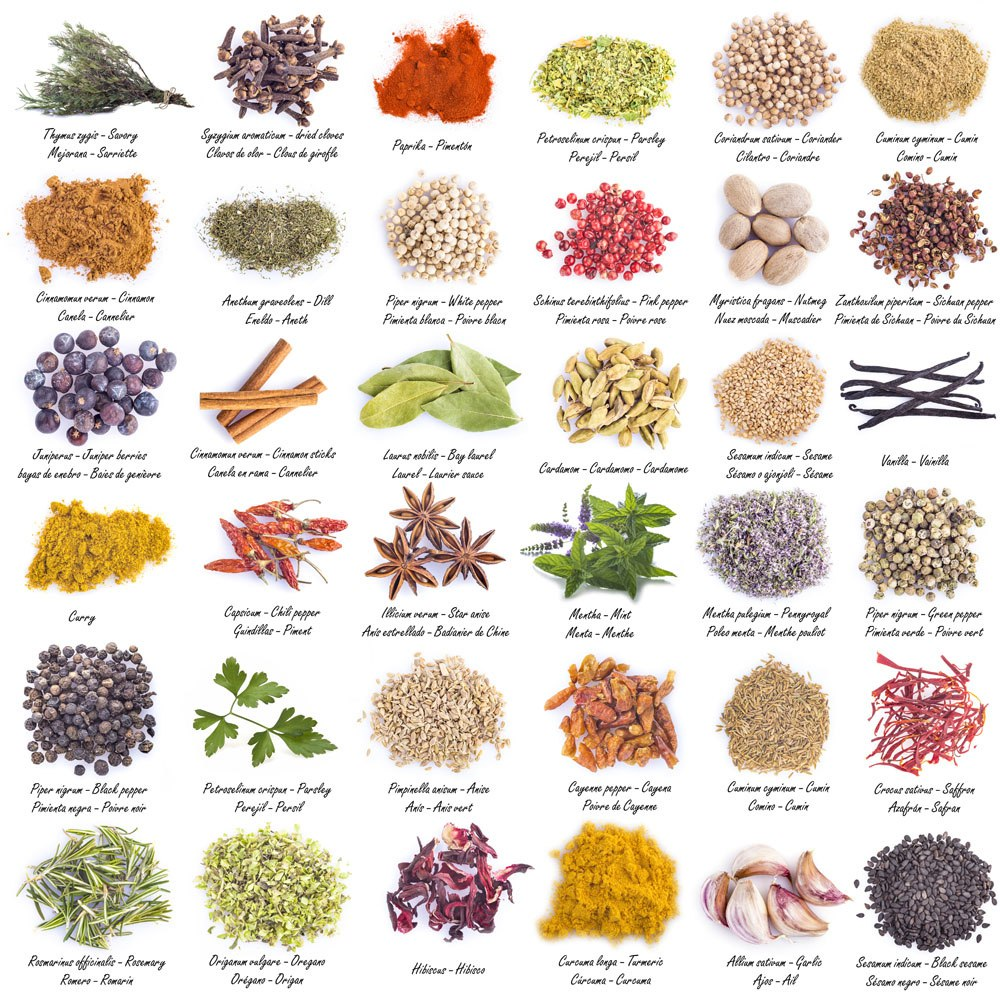
\includegraphics[width=0.99\textwidth]{Spices}
\end{figure} 
Часто люди путаются при покупке, потому что одна и та же специя может называться по-разному. \paragraph{Приведу синонимы самых ходовых}
\begin{itemize}

\item Зира = Кумин
\item Эстрагон = Тархун
\item Базилик = Реган
\item Кориандр = Семена кинзы
\item Тимьян = Чабрец
\item Пажитник голубой = Донник = Уцхо-сунели
\item Пажитник сенной = Шамбала
\item Орегано = Душица (род Origanum)
\item Кондари = Чабер
\item Бадьян = Анис звёздчатый
\item Солодка = Лакрица
\item Мелисса = Лимонная мята
\item Чили = Кайенский перец
\item Чёрный тмин = Калинджи = Чернушка
\item Каркадэ = Гибискус

\end{itemize}
\paragraph{Несколько фактов на заметку}
\begin{itemize}
\item  Чабер и чабрец — два разных растения.
\item  Узбекские лепёшки посыпают кунжутом и чёрным тмином.
\item То, что продают на рынке под видом листьев шафрана, на самом деле листья бархатцев. Настоящий шафран в сотни раз дороже.
\item Анис, фенхель и тмин имеют разные свойства, но похожие ароматы.
\item Ванильный сахар без натуральной ванили — это химия.
\item Не путайте кумин и тмин — это разные растения.
\item Не путайте гималайскую розовую соль и индийскую пахучую розовую соль.
\end{itemize}

\subsection{Как отличить хорошие специи и приправы от поддельных}
А вот \href{https://shrtm.nu/spice}{любопытная статейка про пряности}, так сказать, ликбез для чайников.
Ниже приведена выдержка из нее.
\begin{quote}\emph{
Несколько лет назад в Самарской области из продажи изъяли большую партию молотого красного перца, в которой помимо посторонних механических примесей были обнаружены бактерии сальмонеллы. А под «механическими примесями» скрывался толченый кирпич. И это лишь один из множества случаев, ставших достоянием общественности. Можно ли настоящие специи отличить от поддельных?
%
\paragraph{Цена доверия.}\ Повар придорожной закусочной Заза, долгие годы доставлявший специи из Грузии в Россию, уверяет, что в любую молотую пряность можно добавить что угодно:
\\
-- Главное, чтобы это было мелким, – Заза шевелит пальцами в воздухе, изображая сыпучесть примеси. – Песок там, зола, пыль, труха из мешка. Цвет? Ну, зола – для черного перца, кирпич – для красного. Мука? Мука – это дорого. Но тоже сойдет, если нечего больше. А вообще-то я для себя никогда здесь специй не покупаю. Ни на рынке, ни в магазине. Мне их отец привозит, из Грузии. 
\\
--- А правда, что семена бархатцев на рынке подсовывают вместо шафрана? Как их можно различить?
\\
--- Ты кто – ботаник, шеф-повар? Нет? Тогда никак не различишь.
\\
--- А по цене?
\\
--- Шафран не будут на рынке продавать по 200 рублей за грамм. Никто не купит. А он так примерно и стоит – если настоящий.
--- Ты не представляешь, что в мешках с цельными пряностями может попадаться – и дохлые жуки-червяки, и мышиный помет, и шерсть, и земля. /\ldots/ В молотые (в магазинных пряностях)~--- вполне может что-то попадать. Но там все-таки спецобработка проводится, не заболеешь хотя бы. А на рынке… Сама же видела, как там пряности из открытых мешков в газетные кулечки пересыпают. Мой совет: если купила такое, то не сыпь в готовое блюдо. Добавляй во время варки-жарки – все-таки термическая обработка.
\\
--- А как определить, есть ли в специи нежелательные примеси?
\\
--- Кинь щепотку пряности в воду и размешай. Кирпич, песок выпадут в осадок. От муки или крахмала будет помутнение раствора. А что дальше делать с такой специей – тебе решать.
\\
--- А почему у рыночных пряностей все-таки более сильный аромат?
\\
--- Во-первых, продавцы смалывают их все-таки не за год до продажи, а «поближе к делу». Во-вторых, чем больше пряности в мешке, тем сильнее ее запах.
%
\paragraph{Слагаемое цены.}\ В магазинах пряности дороже, спору нет. Но нельзя забывать, из чего складывается эта дороговизна. Цена на пакетики со специями зависит от стоимости исходного сырья, 99 процентов которого завозится из-за рубежа, что, разумеется, влияет на ценообразование – это во-первых. Некоторые пряности – укроп, петрушка, чеснок, паприка – выращиваются и в России. Но, как отмечают менеджеры компаний-производителей, наши поставщики пока не способны конкурировать с зарубежными ни по качеству, ни по количеству даже таких простых видов пряного сырья. 
\\
Во-вторых, чтобы сырье удовлетворяло всем нормам, в ходе промышленной обработки его особым образом стерилизуют – так, чтобы болезнетворные микробы погибли, но сами специи своих вкусовых и ароматических свойств не потеряли. Использование подобных технологий и весьма недешевого оборудования также сказывается на конечной цене продукта. 
\\
К счастью, в наше время пряности уже не ценятся на вес золота. Однако основным критерием их качества по-прежнему является правило: чем пряность дешевле, тем меньше в ней пряности. И ничего с этим не поделать.
    }
\end{quote}

Берите пряности только в специализированных магазинах и в закрытой упаковке!

\section{Как обжаривать специи}

Нежно берёте специю и жарите чувственно и с любовью до лёгкого румянца \faHeart! 
Обычно на топлёнке.
\paragraph{Разница только во времени}
\begin{itemize}
\item Горчица: до тех пор, пока не будет потрескивать и выпрыгивать из сковороды.
\item Кумин: 10-20 сек до раскрытия аромата. Не пережаривайте после потемнения — может горчить.
\item Имбирь тёртый: 20 сек до румянца.
\item Чеснок: 20 сек до румянца.
\item Чили в стручках: семена в сторону, жарим только кожуру.
\item Корица в палках: 1 минута или до раскрытия аромата.
\item Гвоздика целая: до раскрытия аромата.
\end{itemize}

Молотые, такие как куркума или асафетида лучше добавлять непосредственно перед закладкой овощей, к примеру, чтобы отдать маслу вкус, цвет и аромат, которое потом пропитает ингредиенты. Долго не жарьте — могут сгореть.

Если блюдо не предполагает наличие масла (напр. пряный напиток), можно обжарить на сухой сковороде.

\textbf{Совет дня:} не смешивайте разные марки специй. Выбрали одну — с ней и работайте.

Удачи в экспериментах!


\section{Коварство специй}\label{sec:replace}

Конечно, специи помогают сделать блюдо более привлекательным, но есть специи откровенно вредные, которым следует найти замену, и к ним относятся:
\begin{itemize}
\item Сахар рафинад
\item Соль поваренная
\item Уксус
\item Соевый соус
\item прочие редкие экземпляры
\end{itemize}

\paragraph{Чем заменить?}

\subsection{Сахар}

— смело замещается мёдом. Это вкуснее и полезнее.
Если мёд вызывает у вас аллергию, найдите себе акациевый. Если он у вас вообще вызывает отторжение, значит либо разоряться на альтернативу, типа сиропа агавы, топинамбура, виноградного сиропа или шелковицы, либо нужно чиститься, что предпочтительней, потому что аллергия — это всего лишь естественный катализатор процессов очищения. Миф про обделённых пчёлок — фуфло — ешьте с радостью и столько, сколько хочется.

Ещё немного про сахар. Сейчас в продаже появился «тростниковый» коричневый сахар — это тоже фуфло, потому что это тот же рафинад с добавлением мелассы — ничего хорошего. Настоящий тростниковый сахар производят несколько фирм, одна из которых под маркой «Сахараджа» — он плотный, ароматный, комковатый, солоноватый и тёмно-коричневого цвета. Но по сути — та же дрянь, что и обычный сахар.

\subsection{Соль}

Это, пожалуй, самый сильный наркотик, и слезть с неё сложнее, чем с некоторых мед препаратов. Самое правильное — исключить полностью и «переболеть». Очень скоро вы почувствуете реальный вкус продуктов, а продержавшись недельки три, употреблять её больше не захочется. Не знаю, насколько это осуществимо для вегетарианцев, и тем более, веганов, но попробовать стоит.
А для заложников вкуса предложу выбирать изначально солёные (т.е. богатые натрием) продукты, например вкусные помидоры, сельдерей, морскую капусту, рожь, фасоль, шпинат, изюм и прочие.
Для ленивых есть ещё одна альтернатива поваренной соли — это т.н. Гималайская соль. Однако под одним и тем же названием продают и гималайскую, и вонючую индийскую. Не скажу, что сильно полезно, т.к. всё равно нарушает водный баланс, но лучше чем выварочная.
Гималайскую можно купить в Перекрёстке или здесь: http://hpcsalt.ru (рекомендую навестить их офис — узнаете много интересного)
Вонючую индийскую — в магазинах специй, но это на любителя, т.к. пахнет варёным яйцом.

\subsection{Уксус}

Его часто используют при консервации и приготовлении соусов. Не знаю, зачем он вообще нужен, если есть лимонный сок. Поэтому лимон, друзья, только лимон! А про консервы забудьте.

\subsection{Соевый соус}

Ещё более опасный наркотик, чем сахар и соль, потому что содержит в себе помимо первых двух, продукт соевого брожения (аналогично с дрожевым хлебом), и возможно глютамат, хоть об этом и не пишут на упаковке. Если и выбирать, то только естественного брожения и в стеклянной бутылке (в стекле обычно без консервантов). Пример — соус Sensoy.

Вообще, вопрос вреда и пользы всегда должен восприниматься в контексте. 
% Подробно на этот вопрос ответил Арсен: https://vk.com/videos2453299?z=video198350997_4562390..

Думайте головой!

\section{Имитация вкуса с помощью специй}

Есть чем поделиться, поскольку набралось несколько любопытных рецептов. Будет интересно тем, кто не может отказаться от колбасы, сыра или печенья. Начнём:

\subsection{Колбаса}

Благодаря каналу Михаила, мы поняли, что веганская колбаса по вкусу ничем не отличается от магазинной «мясной». Отсюда следует, что всё дело преимущественно в специях. Несколько вариантов на выбор:

\begin{itemize}
\item Мускат + кориандр + душистый перец + чеснок + соль.
\item Асафетида (чеснок для особо просветлённых) + паприка + мускатный орех + черный перец.
\item Пажитник + паприка + чили + корица + чеснок + черный перец.
\item Мускат + кориандр + душистый перец + кардамон
\item Перец чёрный + перец душистый + базилик + куркума + паприка
\end{itemize}
Наполнителями могут быть: соя, горох, маш, нут, чечевица, сейтан, адыгейский сыр, тофу и другие. Фалафель, кстати — самый яркий представитель альтернативы мясу. Рецепты этих блюд ищите сами. Экспериментируйте, пока не надоест.

\subsection{Сыр}

Заменить этот наркотик можно перейдя сначала на безсычужную брынзу, затем на Адыгейский, а также найдя экологичную замену в виде следующих рецептов на выбор:
\begin{itemize}
    \item \hyperref[aiolli]{Соус Айолли}~---  отлично сочетается с помидорами, прямо новогодняя тема!

\item \hyperref[takini]{Соус Тахини}~--- получается плотно, по вкусу прямо как сыр — можно на хлебцы намазывать.
\end{itemize}


\subsection{Печенье}

\hyperref[cookies]{Рецепт} нашёлся случайно. Жирненько, сладенько, пахнет выпечкой. По вкусу, как песочное тесто.

\subsection{Грибы}

Смело заменяется листьями пажитника — офигенная штука! Чем плохи грибы?~--- ничем, просто это не еда.

\subsection{Шоколад}

Урбеч из тёмного льна + мёд.

\subsection{Майонез}
\begin{itemize}
\item Подсолнечные семечки + вода + соль + лимонный сок + чеснок — в блендер.
\end{itemize}

Здравия и благоразумия!

